\documentclass[11pt,twocolumn]{article}
\usepackage[utf8]{inputenc}
\usepackage{times}
\usepackage{geometry}
\geometry{a4paper,margin=1in}

\usepackage{hyperref}
\usepackage{url}
\usepackage{booktabs}
\usepackage{multirow}
\usepackage{graphicx}
\usepackage{xcolor}
\usepackage{amsmath}
\usepackage{amsfonts}
\usepackage{amssymb}
\usepackage{xspace}
\usepackage[round]{natbib}
\usepackage{float}
\usepackage{rotating}
\usepackage{placeins}
\usepackage{caption}
\captionsetup{font=small}

\title{Hierarchical NURBS-Inspired Multi-Domain Loss for Training Deep Time-Series Forecasting Models}

\author{Jason Abohwo\thanks{Equal contribution.} \\
Yale University\\
New Haven, CT 06511, USA \\
\texttt{Jason.Abohwo@Yale.edu}\\
\and
Srikara Vishnubhatla\footnotemark[1] \\
Yale University\\
New Haven, CT 06511, USA \\
\texttt{Srikara.Vishnubhatla@Yale.edu}\\
}
\date{}

\newcommand{\methodName}{HNMD\xspace}

\begin{document}

\maketitle

\begin{abstract}
Deep forecasting models are almost universally trained with point-wise objectives such as mean squared error (MSE). Point-wise losses reward matching individual time steps but are indifferent to the multi-scale structure of a series: a forecast can achieve low MSE while misrepresenting local slopes, periodic components, and spectral content. We introduce the \emph{Hierarchical NURBS-Inspired Multi-Domain Loss} (\methodName), a training objective that (i) decomposes predictions and targets into a hierarchy of weighted basis-spline approximations of increasing resolution, inspired by Non-Uniform Rational Basis Splines (NURBS), (ii) compares the two decompositions jointly in the time, derivative, and frequency domains, and (iii) rescales per-level gradients by data-driven level importances during backpropagation. \methodName is architecture-agnostic and changes only the training loss: models, capacity, optimizer, and schedules are held fixed in all comparisons. On nine multivariate long-horizon benchmarks with four prediction lengths each, training a fixed 3-layer MLP with \methodName improves test MSE and MAE over the same model trained with MSE or with the shape-aware TILDE-Q loss on the large majority of dataset--horizon cells, with the largest gains on the hourly ETT benchmarks; gains transfer to DLinear and iTransformer backbones. A component ablation shows that the spline hierarchy, the multi-domain terms, and the gradient weighting each contribute to final accuracy. We release code, experiment configurations, and scripts that reproduce every table and figure.\footnote{\href{https://github.com/srikara-V/Hierarchical-NURBS-Inspired-Multi-Domain-Loss-for-Training-Deep-Time-Series-Forecasting-Models}{\texttt{github.com/srikara-V/Hierarchical-NURBS-}\\\texttt{Inspired-Multi-Domain-Loss-for-Training-}\\\texttt{Deep-Time-Series-Forecasting-Models}}}
\end{abstract}

\section{Introduction}
\label{sec:intro}

Time-series forecasting (TSF) underpins decision making in domains ranging from energy and transportation to finance and healthcare. The field has progressed from classical statistical models such as ARIMA \citep{arima} through recurrent architectures \citep{lstm,gru} to a rapid succession of deep forecasting architectures: decomposition-based and frequency-enhanced Transformers \citep{autoformer,fedformer}, efficient attention variants \citep{informer,reformer,flowformer}, patch-based and inverted Transformers \citep{patchtst,itransformer}, lightweight linear models \citep{dlinear,rlinear,tide}, state-space models \citep{timemachine}, reprogrammed language models \citep{TimeLLM}, and channel-fusion architectures \citep{softs}.

While architectures have evolved quickly, the objective used to train them has remained largely unchanged: almost all of the models above are optimized with mean squared error (MSE) or mean absolute error (MAE). Point-wise objectives are simple and well-conditioned, but they evaluate each time step independently and are therefore blind to the joint structure of the sequence. Deep networks tend to exploit whatever decision rule most easily reduces their training criterion \citep{shortcut}, and gradient descent is biased toward fitting low-frequency structure first \citep{spectralbias}; under a purely point-wise criterion this frequently yields over-smoothed forecasts that track the conditional mean while washing out local shape, sharp transitions, and periodic detail. Prior work on structure-aware objectives confirms the diagnosis: DILATE \citep{dilate} adds differentiable shape and temporal-alignment terms built on soft-DTW \citep{softdtw}, TILDE-Q \citep{tilde-q} designs transformation-invariant terms that tolerate amplitude and phase shifts, and FreDF \citep{fredf} supervises directly in the frequency domain. These objectives each capture one or two specific facets of temporal structure --- warping, invariance, or spectrum --- but none supervises the \emph{multi-scale composition} of a series: the fact that an observed sequence superimposes several dynamics of different complexities, each of which the forecast should reproduce.

We propose the \textbf{Hierarchical NURBS-Inspired Multi-Domain Loss} (\methodName), a training objective built on an explicit multi-scale representation. \methodName decomposes both the prediction and the target into a hierarchy of spline approximations of increasing resolution, using weighted basis splines whose control-point weights are set from regional statistics of the series (inspired by NURBS \citep{piegl}, but with weights assigned by a criterion rather than optimized). The two hierarchies are then compared level-by-level in three domains --- raw values (time), first differences (derivative), and Fourier magnitudes (frequency) --- and, during backpropagation, the gradient contribution of each hierarchy level is rescaled by a data-driven importance derived from that level's current error. Intuitively, \methodName asks the model not only to be right on average, but to be right \emph{at every scale of the series and in every domain in which structure manifests}, focusing learning on the scales where it currently errs most.

\methodName is a pure drop-in replacement for the training criterion. It requires no architectural changes, adds no inference cost, and is applicable to any model trained by gradient descent. We evaluate it as such: for each benchmark we fix the architecture, capacity, optimizer, learning rate, and schedule, and vary \emph{only} the training loss among MSE, TILDE-Q, and \methodName.

Our contributions are:
\begin{itemize}
    \item \textbf{Complexity-based decomposition as a supervision target.} A simple residual scheme that peels a series into components of increasing representational complexity using region-weighted basis splines, giving the loss access to explicit multi-scale structure (Sections~\ref{sec:cbd}--\ref{sec:wsd}).
    \item \textbf{\methodName.} A training objective combining the spline hierarchy with time-, derivative-, and frequency-domain error terms and level-importance gradient weighting (Section~\ref{sec:loss}).
    \item \textbf{Comprehensive evaluation.} Loss-controlled comparisons on nine benchmarks and four horizons against MSE and TILDE-Q training for three architectures (MLP, DLinear, iTransformer), seed-robustness checks, a fixed-configuration variant that removes per-dataset tuning, training-cost measurements, and a component ablation (Section~\ref{sec:experiments}). \methodName wins the large majority of completed dataset--horizon cells on the MLP and transfers to the other backbones.
\end{itemize}

We also report negative aspects candidly: \methodName introduces hyperparameters that benefit from per-dataset tuning, increases training cost per step, and does not close the gap to the strongest specialized architectures on channel-rich datasets when applied to a small MLP (Section~\ref{sec:limitations}).

\section{Related Work}
\label{sec:related}

\subsection{Deep forecasting architectures}
Classical approaches such as ARIMA and seasonal ARIMA \citep{arima,seasonalarima} model a series through differencing and moving averages but struggle with nonlinear dynamics. Recurrent networks \citep{rnn,lstm,gru} improved long-range modeling, and attention-based architectures now dominate the long-horizon setting. Informer \citep{informer} sparsifies attention for long inputs; Autoformer \citep{autoformer} replaces attention with an auto-correlation mechanism over trend/seasonal decompositions; FEDformer \citep{fedformer} mixes frequency-domain representations into the decomposition. PatchTST \citep{patchtst} tokenizes local patches with channel independence; iTransformer \citep{itransformer} inverts the attention axes, attending across variates instead of time; SOFTS \citep{softs} aggregates channels through a shared core representation. In parallel, remarkably simple models --- DLinear \citep{dlinear}, RLinear \citep{rlinear}, TiDE \citep{tide}, and MLP variants --- remain competitive, and state-space (TimeMachine, \citealp{timemachine}) and LLM-reprogramming (Time-LLM, \citealp{TimeLLM}) approaches broaden the design space further. All of these train with point-wise MSE (occasionally MAE). Our work is orthogonal: we keep the architecture fixed and change only the objective.

\subsection{Training objectives for forecasting}
Beyond MSE/MAE and their scale-adjusted relatives (RMSE, MAPE, SMAPE; \citealp{mape}), several objectives target temporal structure explicitly. Soft-DTW \citep{softdtw} makes dynamic time warping differentiable, enabling alignment-aware training; DILATE \citep{dilate} combines a soft-DTW shape term with a temporal-distortion penalty so that both the geometry and the timing of events are supervised. TILDE-Q \citep{tilde-q} constructs three terms that are invariant to amplitude shift, phase shift, and uniform amplification, using softmax-normalized signed distances, dominant Fourier coefficients, and normalized cross-correlation. FreDF \citep{fredf} shows that computing the error in the frequency domain mitigates the effect of label autocorrelation. \methodName differs from this line of work along two axes. First, rather than making the loss \emph{invariant} to selected transformations or moving it into a single alternative domain, \methodName supervises an explicit \emph{hierarchy} of series components, so that coarse trajectory and fine detail receive separate, weighted supervision. Second, its three domain terms act on that shared decomposition rather than on the raw series, which couples multi-domain supervision with multi-scale structure. We compare against TILDE-Q as the strongest recent representative of shape-aware losses, and against MSE as the standard.

\section{Preliminaries}
\label{sec:prelim}

\subsection{Multivariate long-horizon forecasting}
Given a look-back window $X = \{x_1,\dots,x_L\} \in \mathbb{R}^{L \times C}$ of $L$ steps and $C$ variates, a forecaster $f_\theta$ predicts the next $T$ steps $\hat{Y} = f_\theta(X) \in \mathbb{R}^{T \times C}$, with ground truth $Y \in \mathbb{R}^{T \times C}$. Training minimizes $\mathcal{L}(\hat{Y}, Y)$ over a dataset of sliding windows; the canonical choice is $\mathcal{L}_{\mathrm{MSE}} = \frac{1}{TC}\lVert \hat{Y} - Y \rVert_2^2$. Following \citet{tilde-q}, we use \emph{temporal dynamics} informally for the informative periodic and non-periodic patterns of a series (trends, peaks, dips, oscillations); any given series may superimpose $m$ distinct such dynamics.

\subsection{B-splines and NURBS}
A spline is a piecewise-polynomial function whose pieces join at a non-decreasing sequence of knots $t_0 \le t_1 \le \dots \le t_n$. B-splines form a convenient basis for the space of splines of a given degree: the basis functions $B_{i,k}$ are defined by the Cox--de Boor recursion \citep{deboor}
\begin{equation}
B_{i,0}(u) = \begin{cases} 1 & t_i \leq u < t_{i+1} \\ 0 & \text{otherwise,} \end{cases}
\end{equation}
\begin{equation}
\begin{split}
B_{i,k}(u) &= \frac{u - t_i}{t_{i+k} - t_i} B_{i,k-1}(u) \\
&\quad + \frac{t_{i+k+1} - u}{t_{i+k+1} - t_{i+1}} B_{i+1,k-1}(u).
\end{split}
\end{equation}
A series $y(u)$ is approximated as $y(u) \approx \sum_i c_i B_{i,d}(u)$ with coefficients fit by least squares. The density of the knot vector controls the resolution of the approximation: few knots yield smooth, low-complexity fits; many knots resolve fine detail.

Non-Uniform Rational B-Splines (NURBS; \citealp{piegl}) generalize B-splines by attaching a weight $w_i$ to each control point,
\begin{equation}
\label{eq:nurbs}
N_{i,d}(u) = \frac{w_i\, B_{i,d}(u)}{\sum_{j} w_j\, B_{j,d}(u)},
\end{equation}
so that regions with larger weights attract the curve more strongly. In computer-aided design both the control points and the weights are optimized. In this work the weights are instead \emph{assigned} from a regional statistic of the data (Section~\ref{sec:wsd}), which biases the basis toward regions selected by that statistic without the cost or instability of weight optimization.

\section{Method}
\label{sec:method}

\methodName has three parts: a residual decomposition scheme that produces a hierarchy of approximations (\ref{sec:cbd}); its instantiation with regionally weighted basis splines (\ref{sec:wsd}); and the loss itself --- multi-domain comparison of the decomposed prediction and target with level-weighted gradients (\ref{sec:loss}). Figure~\ref{fig:overview} summarizes the pipeline.

\begin{figure*}[!t]
\centering
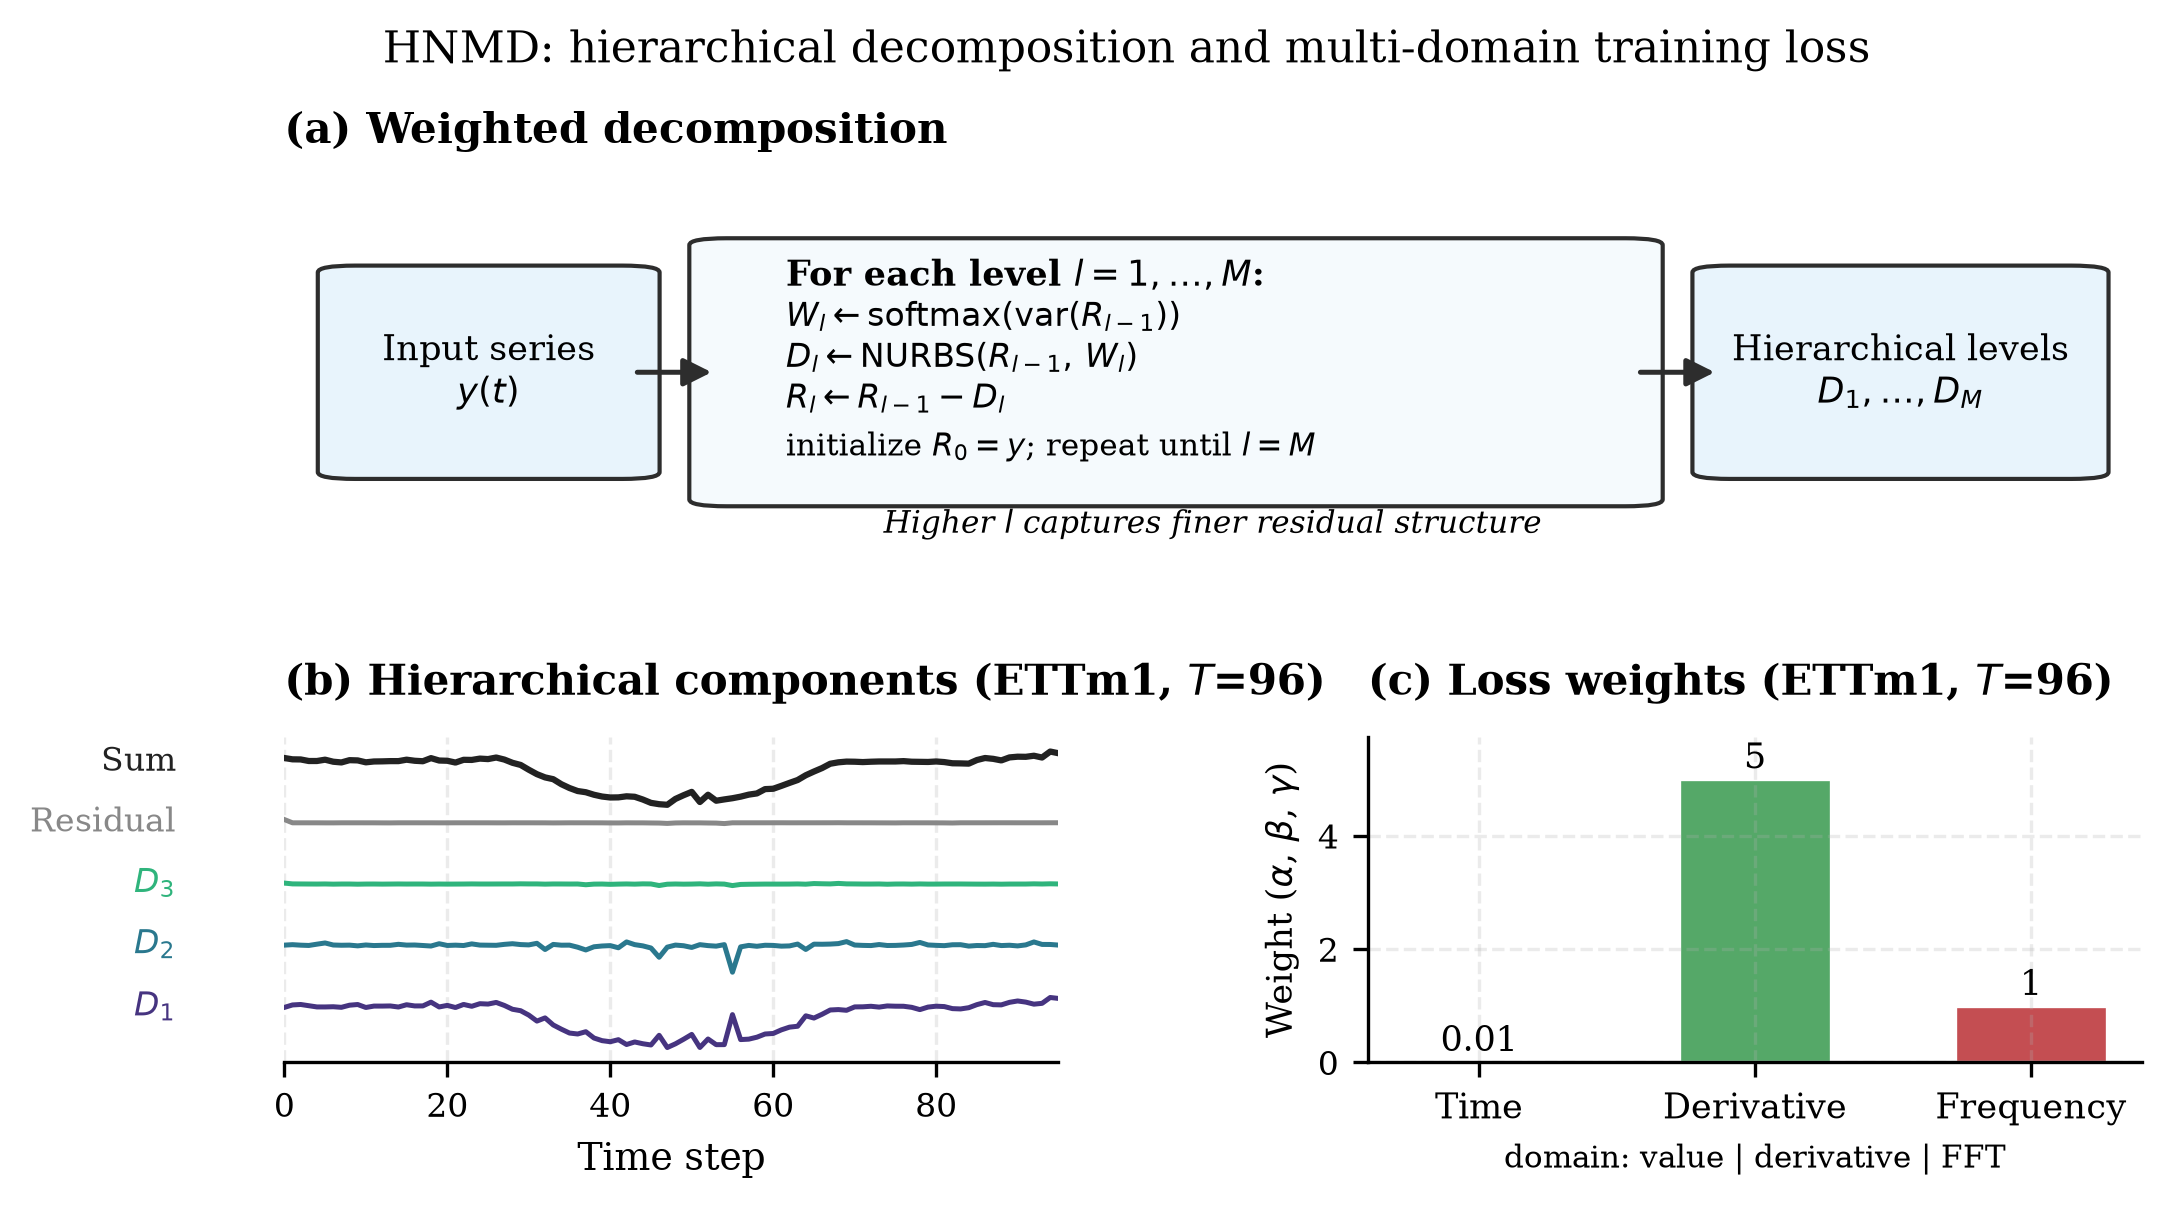
\includegraphics[width=0.98\textwidth]{figures/fig1_method_overview.png}
\caption{\methodName overview. Prediction and target are each decomposed into a hierarchy of weighted-spline components of increasing resolution; the two hierarchies are compared in the time, derivative, and frequency domains, and per-level gradient contributions are rescaled by data-driven importances during backpropagation.}
\label{fig:overview}
\end{figure*}

\subsection{Complexity-based decomposition}
\label{sec:cbd}

Let $y(t)$ superimpose $m$ latent dynamics of differing complexity, where we take the \emph{complexity} $q(\cdot)$ of a component informally as the representational capacity (e.g., number of spline coefficients) required to approximate it well. Given a family of function approximators $f_1, \dots, f_M$ of increasing capacity $r(f_1) < \dots < r(f_M)$, we define the decomposition recursively on residuals:
\begin{align}
R_0(t) &= y(t), \\
\hat{f}_i(t) &= \arg\min_{f_i} \; \lVert R_{i-1} - f_i \rVert^2, \\
R_i(t) &= R_{i-1}(t) - \hat{f}_i(t), \qquad i = 1,\dots,M,
\end{align}
so that $y(t) = \sum_{i=1}^{M} \hat{f}_i(t) + R_M(t)$. Each level fits only what previous, simpler levels could not express: level~1 captures the coarsest attainable structure, level~2 the coarsest structure of the remainder, and so on. If $M = m$ and the capacities align with the latent complexities ($r(f_i) = q_i$ for each $i$), the levels isolate the individual dynamics; in the realistic case $M \neq m$, each level captures a \emph{group} of dynamics of neighboring complexity. For the purposes of a loss function exact separation is not required --- what matters is that the hierarchy exposes coarse-to-fine structure as separate, individually supervisable components.

\subsection{Weighted spline decomposition}
\label{sec:wsd}

We instantiate the approximators with basis splines of degree $d=3$ whose knot counts grow with the level, and bias each fit toward high-variance regions through NURBS-style weights. For a window of length $T$ (the prediction horizon) and level $l = 1, \dots, M$:

\textbf{(1) Knot vector.} Level $l$ uses $K_l = \kappa \cdot \max\!\big(2d + 2,\ \min(T/2,\ 2^{\,l+1} + T/6)\big)$ uniformly spaced knots on $[0, T]$, where $\kappa$ is a global \emph{knot multiplier} hyperparameter. $K_l$ increases with $l$, so each level has strictly more resolution than the last.

\textbf{(2) Regional weights.} From the current residual $R_{l-1}$ we compute a sliding-window variance with window size $\lfloor T / K_l \rfloor$ and softmax-normalize it along time:
\begin{equation}
W_l = \operatorname{softmax}_t \big( \operatorname{Var}_{\mathrm{win}}(R_{l-1}) \big),
\end{equation}
which concentrates basis mass where the residual is most active. The weighted (NURBS-style) basis follows Eq.~\eqref{eq:nurbs} with $W_l$ in place of the optimized weights; for efficiency the weighted basis of each level is computed once and cached, so the weights act as a fixed, data-initialized modulation of the basis rather than a per-batch computation (Section~\ref{sec:impl}).

\textbf{(3) Regularized fit and residual update.} With basis matrix $\mathbf{N}_l \in \mathbb{R}^{K'_l \times T}$ ($K'_l = K_l - d - 1$ basis functions), coefficients for all series in the batch are obtained in closed form by ridge-regularized least squares,
\begin{equation}
\mathbf{C}_l = (\mathbf{N}_l \mathbf{N}_l^{\top} + \lambda I)^{-1} \mathbf{N}_l\, R_{l-1}, \quad \lambda = 10^{-6},
\end{equation}
giving the level component $\mathbf{D}_l = \mathbf{N}_l^{\top} \mathbf{C}_l$ and residual $R_l = R_{l-1} - \mathbf{D}_l$.

Finally, the $M$ level components are augmented with the $M-1$ sums of adjacent levels, $\mathbf{D}_l + \mathbf{D}_{l+1}$, yielding a stack $S(y) \in \mathbb{R}^{T \times C \times (2M-1)}$. The adjacent-pair channels couple neighboring scales, so reconstruction quality across scale boundaries is supervised in addition to each scale in isolation. Figure~\ref{fig:decomposition} shows a decomposition of an ETTm1 window: early levels carry the low-frequency trajectory and later levels increasingly fine corrections.

\begin{figure}[!t]
\centering
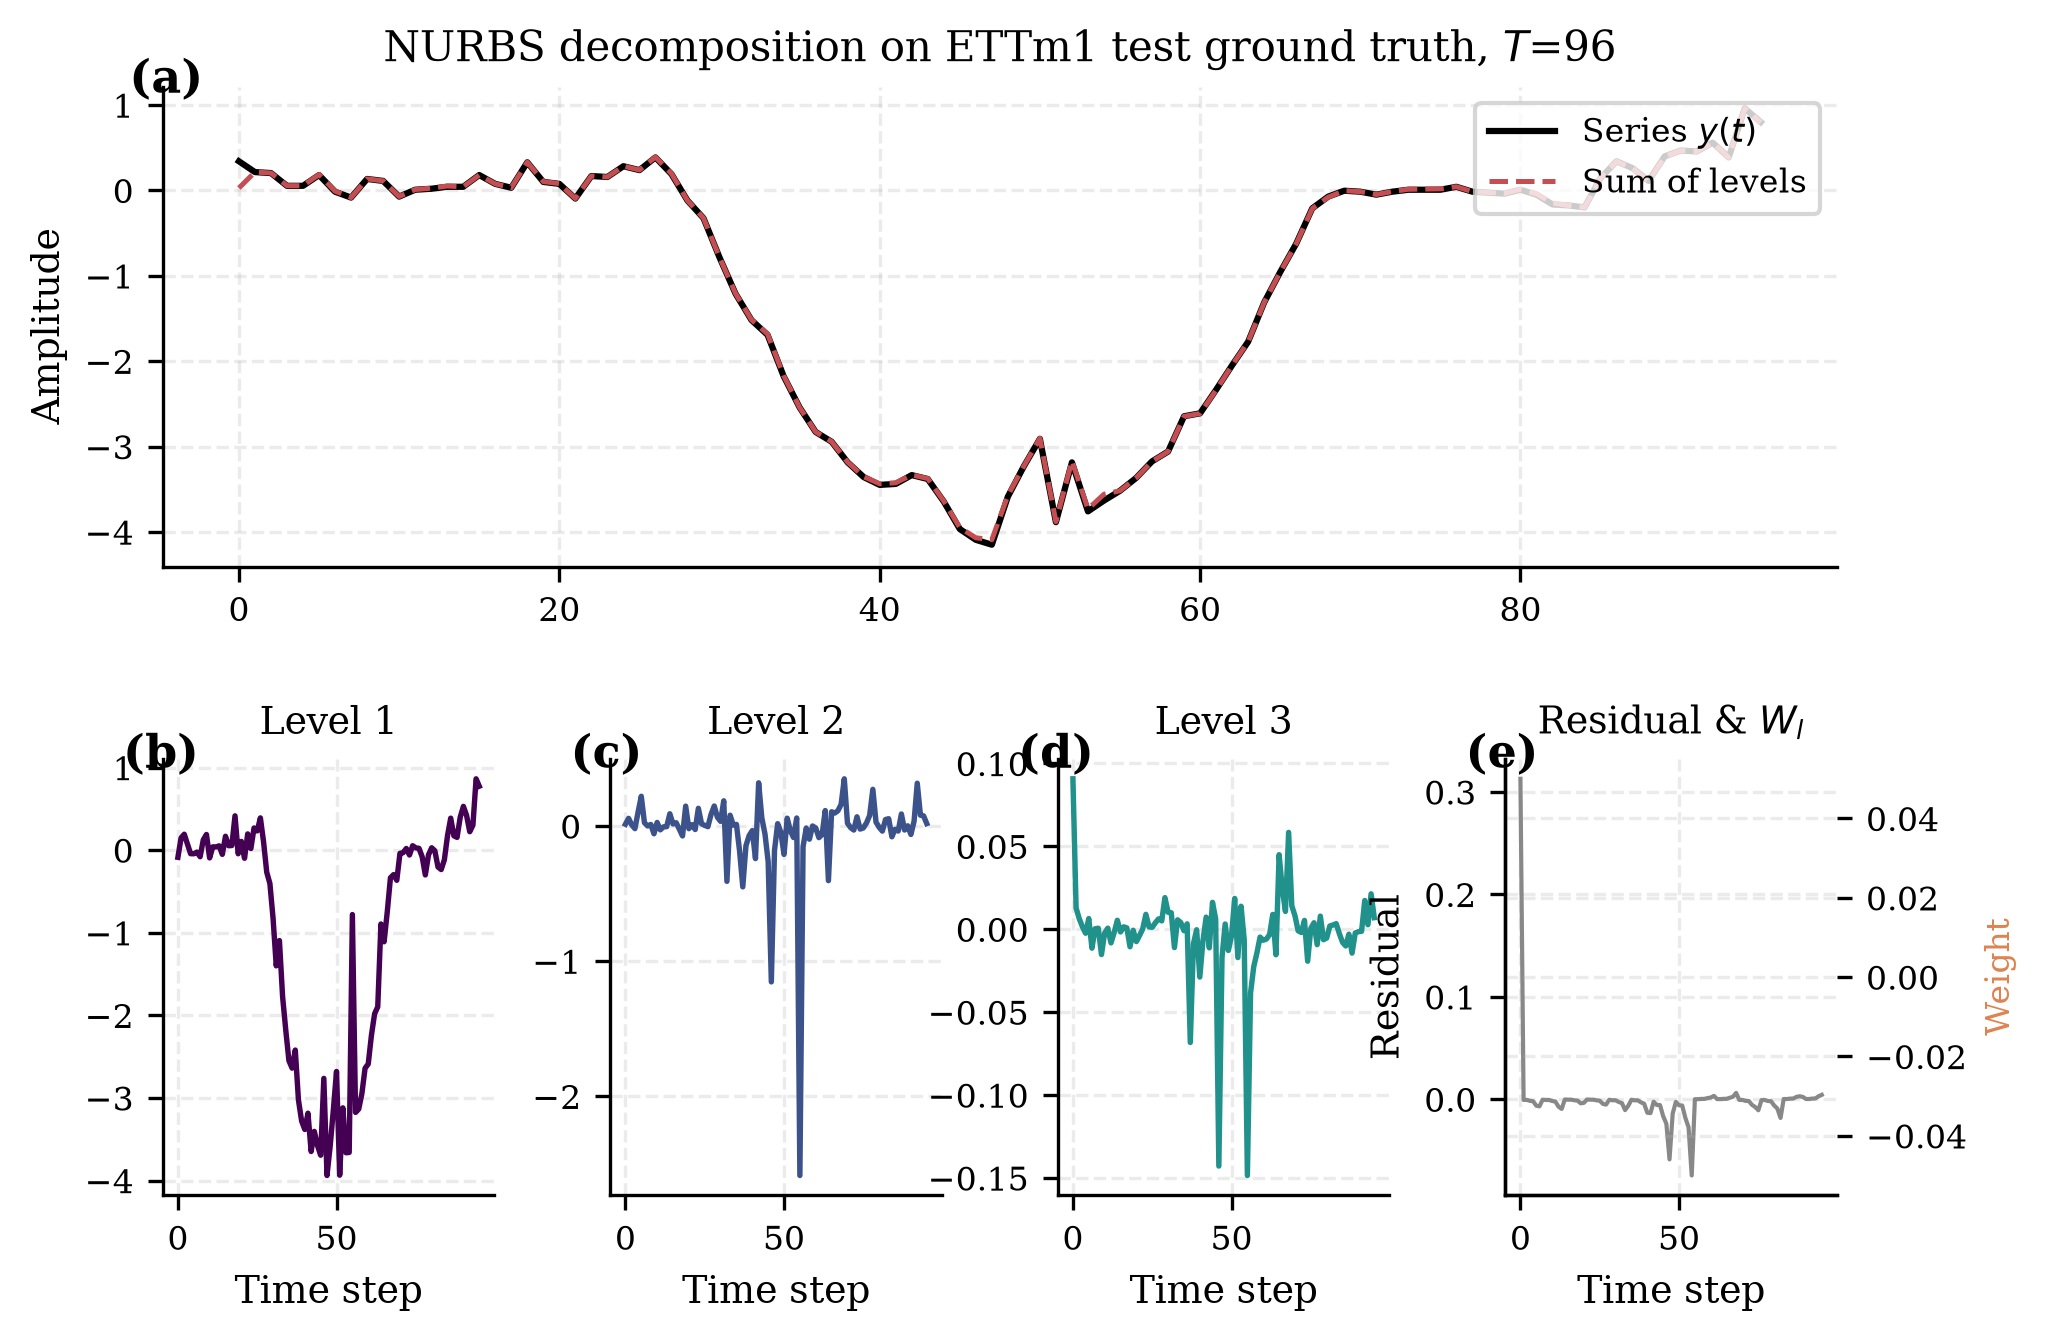
\includegraphics[width=\columnwidth]{figures/fig2_decomposition.png}
\caption{Weighted spline decomposition of an ETTm1 test window (horizon 96). Top: input series and reconstruction; lower panels: hierarchy levels of increasing resolution.}
\label{fig:decomposition}
\end{figure}

\subsection{Level-weighted multi-domain error}
\label{sec:loss}

\textbf{Forward pass.} Both prediction and target are decomposed with the \emph{same} basis (the target's decomposition requires no gradients), giving $s_{\mathrm{pred}} = S(\hat{Y})$ and $s_{\mathrm{true}} = S(Y)$. The loss compares the stacks in three domains:
\begin{equation}
\label{eq:loss}
\begin{split}
\mathcal{L}_{\methodName} ={}& \alpha \, \big\lVert s^{*}_{\mathrm{pred}} - s^{*}_{\mathrm{true}} \big\rVert_1 \\
&+ \beta \, \big\lVert (s'_{\mathrm{pred}})^{*} - (s'_{\mathrm{true}})^{*} \big\rVert_1 \\
&+ \gamma \, \big\lVert \mathcal{F}(s_{\mathrm{pred}})^{*} - \mathcal{F}(s_{\mathrm{true}})^{*} \big\rVert_1,
\end{split}
\end{equation}
where $\lVert\cdot\rVert_1$ denotes the mean absolute deviation over all entries, $'$ is the first difference along time, $\mathcal{F}$ the real FFT along time, and $*$ min--max normalization using global statistics of the training set (value range for the time term, difference range for the derivative term, magnitude range for the frequency term), computed once before training. The normalization places the three domains on comparable scales so that $\alpha, \beta, \gamma$ express genuine trade-offs rather than unit corrections. The time term penalizes displacement of each component; the derivative term penalizes wrong local slopes (over-smoothing and lagged forecasts); the frequency term takes the modulus of the \emph{complex} coefficient difference, so both the amplitude and the phase of each frequency component are supervised. Figure~\ref{fig:multidomain} visualizes the three views for a sample forecast.

\textbf{Backward pass: level-importance weighting.} Levels differ in how much they currently contribute to the error, and uniformly backpropagating through the stack lets easy levels dominate. We therefore rescale gradients per level. During the forward decomposition of the prediction we record, for each of the $2M-1$ stack channels $j$, the importance
\begin{equation}
\iota_j = \operatorname{mean}\big( \lvert s_{\mathrm{pred},j} - s_{\mathrm{true},j} \rvert^{\,x} \big),
\qquad
\omega_j = \frac{\iota_j}{\sum_k \iota_k},
\end{equation}
with exponent $x$ a hyperparameter. In the backward pass, the gradient flowing through stack channel $j$ is multiplied by $\omega_j$ before being accumulated onto the prediction (implemented as a custom autograd node). Larger $x$ concentrates learning on the worst-fit levels; $x = 0$ recovers uniform weighting. Figure~\ref{fig:gradweights} shows the resulting weights on an example: mid-resolution levels carrying mismatched structure receive the largest share of gradient.

\begin{figure}[!t]
\centering
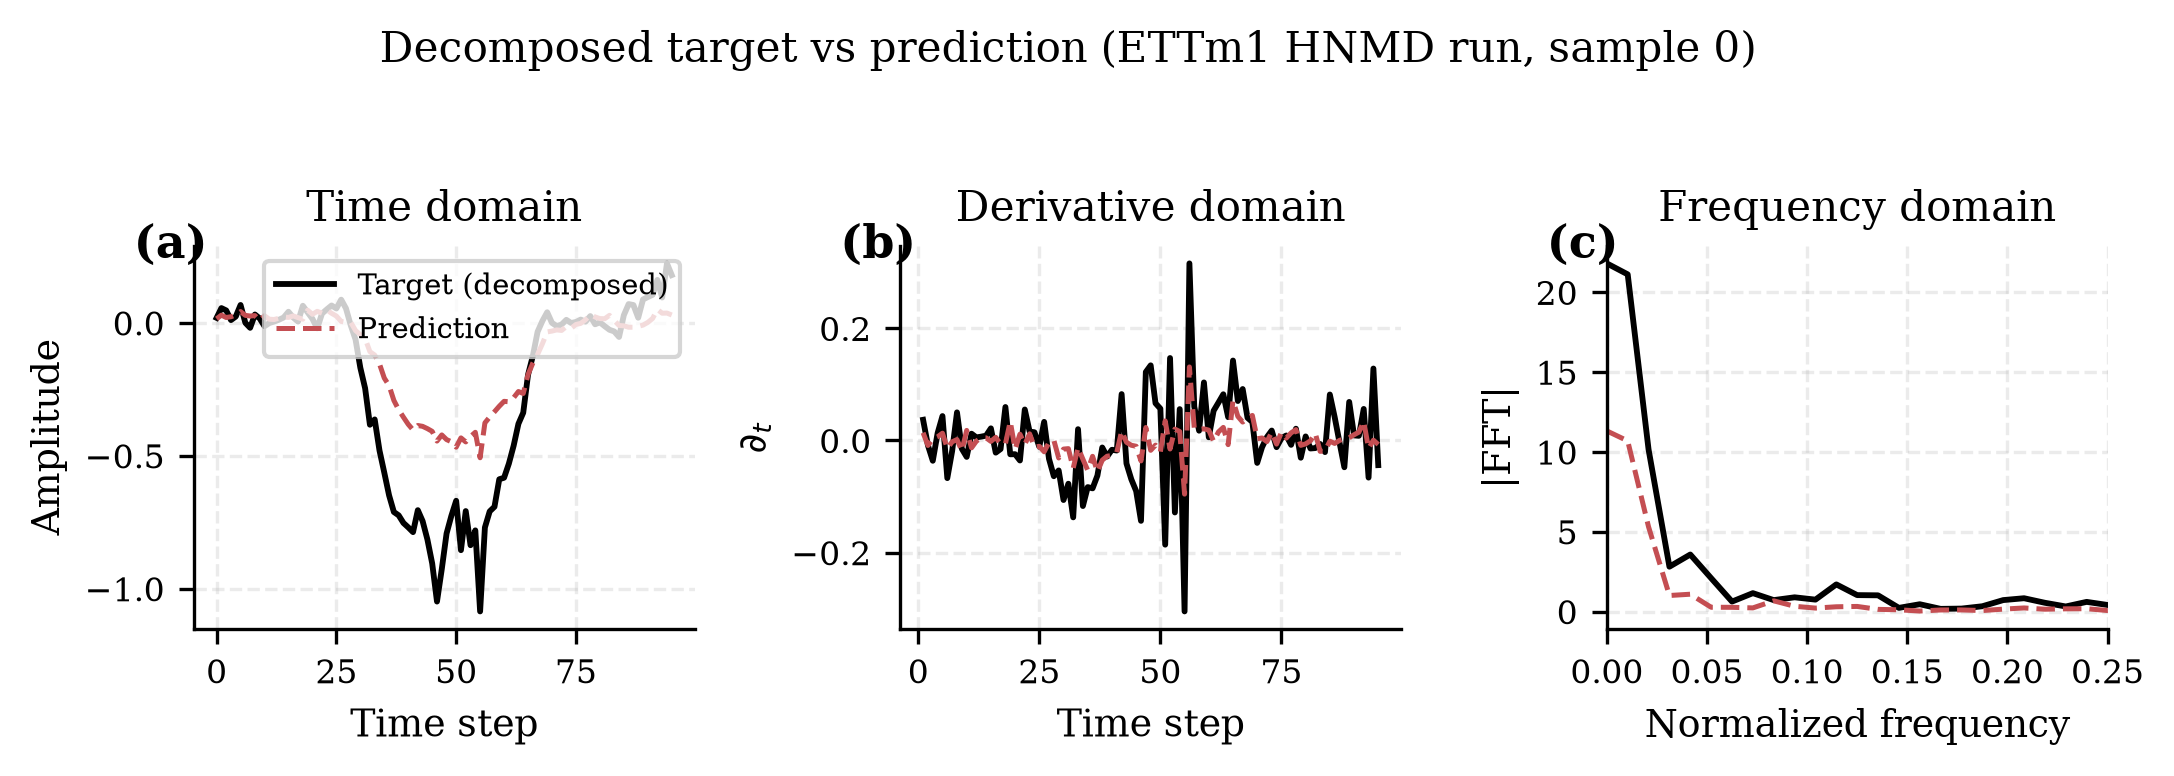
\includegraphics[width=\columnwidth]{figures/fig3_multidomain.png}
\caption{Multi-domain comparison of a decomposed target and prediction: time-domain components, first differences, and FFT magnitudes. A forecast may match in one view while erring in another; \methodName supervises all three.}
\label{fig:multidomain}
\end{figure}

\subsection{Implementation notes and complexity}
\label{sec:impl}

All operations are batched tensor ops on GPU. For batch size $B$, the level-$l$ fit solves one $K'_l \times K'_l$ system with $BC$ right-hand sides; total forward cost is $O\!\big(\sum_l (K_l'^3 + K_l'^2\, T + K_l'\, T\, BC)\big)$, which is dominated in practice by the FFT and elementwise terms for small $K'_l$. The weighted basis of each level is cached after first computation and reused across batches, so the spline weights are data-initialized constants rather than per-batch variables; recomputing them per batch did not change results perceptibly but increases cost. The decomposition is applied to windows of the prediction horizon only (never the look-back), and no component of \methodName is used at inference time --- the deployed model is unchanged. Section~\ref{sec:overhead} quantifies training overhead. The full procedure is $\sim$200 lines of PyTorch; pseudocode is given in Appendix~\ref{app:algo}.

\section{Experiments}
\label{sec:experiments}

\subsection{Setup}
\label{sec:setup}

\textbf{Datasets.} We use nine standard multivariate benchmarks: ETTh1/ETTh2/ETTm1/ETTm2 (electricity-transformer temperature at hourly and 15-minute resolution), Electricity (ECL), Traffic, Weather, Exchange-Rate, and Solar-Energy, with the customary chronological train/val/test splits \citep{autoformer,itransformer}. Details are in Appendix~\ref{app:datasets}.

\textbf{Protocol.} Input length is $96$; prediction lengths are $T \in \{96, 192, 336, 720\}$. Metrics are test MSE and MAE on standardized data (lower is better). Within each comparison, the architecture, capacity, optimizer (Adam, \citealp{kingma2014adam}), learning rate, batch size, schedule, early stopping, and seed are identical across losses --- \emph{only the training criterion changes}. Models are trained for 10 epochs with early stopping (patience 3) on validation loss, following the iTransformer benchmark configuration \citep{itransformer}.

\textbf{Architectures.} Our primary model is a fixed 3-layer MLP (hidden width 512, GELU) applied per variate along time --- a deliberately simple backbone that isolates the effect of the objective. We additionally train DLinear \citep{dlinear} and iTransformer \citep{itransformer} to test transfer across architecture families (linear, attention-based).

\textbf{Losses.} MSE; TILDE-Q \citep{tilde-q} with its published formulation and default weights; and \methodName. \methodName hyperparameters $(\alpha, \beta, \gamma, \kappa, x)$ were selected per dataset and horizon by a small grid search with the MLP ($\approx$7 configurations per cell; Appendix~\ref{app:hyper}); $M{=}5$ and $d{=}3$ are fixed throughout. DLinear uses configurations tuned for DLinear; iTransformer reuses the MLP-tuned configurations unchanged. To quantify how much per-cell tuning matters we also report a \emph{single fixed configuration} shared by all datasets and horizons (Section~\ref{sec:robustness}), and Section~\ref{sec:limitations} discusses the tuning protocol's limitations.

\textbf{Infrastructure.} All runs execute in a single reproducible pipeline (config-driven runner, checkpoint/resume, result aggregation) on NVIDIA L4 GPUs; every number in every table is written by scripts directly from the archived run outputs.

\subsection{Main results: fixed MLP, varying loss}
\label{sec:main-results}

Table~\ref{tab:main} reports the full comparison. Three observations stand out.

\textbf{\methodName improves the majority of cells.} Counting horizon-level firsts by test MSE, \methodName leads in most of the 36 dataset--horizon cells, with MSE training and TILDE-Q splitting the remainder (exact counts in the last row of Table~\ref{tab:main}). Improvements hold on both metrics, indicating genuinely better point forecasts rather than a metric-specific artifact.

\textbf{Gains concentrate where multi-scale structure dominates.} The hourly ETT benchmarks improve most: dataset-average MSE drops by roughly 5--10\% relative to MSE training, and the margin grows with horizon --- precisely the regime where point-wise training over-smooths. On the 15-minute ETT variants gains are consistent but smaller.

\textbf{Channel-rich datasets are harder.} On ECL, Traffic, and Solar (321--862 variates), \methodName is comparable to the best competing loss rather than clearly ahead: differences between all three losses shrink. We attribute this to two factors: a small per-variate MLP is capacity-limited on these datasets regardless of objective, and the shared decomposition basis (computed from the first variate's regional weights) is a coarser fit when hundreds of heterogeneous channels are decomposed jointly.

\begin{table}[!t]
    \centering
    \caption{Multivariate long-horizon forecasting with a fixed 3-layer MLP trained under each loss. Input length is 96 and results are test-set MSE/MAE (lower is better) with prediction lengths $\{96,192,336,720\}$; Avg is the mean over the four horizons. \textbf{Bold} marks the best value in each row. The final row counts horizon-level firsts by test MSE / MAE across all 20 completed dataset--horizon cells.}
    \label{tab:main}
    \scriptsize
    \setlength{\tabcolsep}{2.6pt}
    \renewcommand{\arraystretch}{0.9}
    \begin{tabular}{c|c|cc|cc|cc}
    \toprule
    \multicolumn{2}{c|}{Training loss} &
    \multicolumn{2}{c|}{MSE} &
    \multicolumn{2}{c|}{TILDE-Q} &
    \multicolumn{2}{c}{HNMD (ours)} \\
    \multicolumn{2}{c|}{Metric} &
    MSE & MAE & MSE & MAE & MSE & MAE \\
    \midrule
\multirow{5}{*}{\rotatebox{90}{ETTm1}}
 & 96 & 0.347 & 0.381 & 0.347 & 0.372 & \textbf{0.327} & \textbf{0.364} \\
 & 192 & 0.379 & 0.401 & 0.386 & 0.397 & \textbf{0.366} & \textbf{0.383} \\
 & 336 & 0.429 & 0.442 & 0.420 & 0.423 & \textbf{0.402} & \textbf{0.409} \\
 & 720 & 0.473 & 0.466 & 0.467 & 0.452 & \textbf{0.459} & \textbf{0.448} \\
 \cmidrule(lr){2-8}
 & Avg & 0.407 & 0.422 & 0.405 & 0.411 & \textbf{0.389} & \textbf{0.401} \\
\midrule
\multirow{5}{*}{\rotatebox{90}{ETTm2}}
 & 96 & 0.192 & 0.277 & \textbf{0.184} & \textbf{0.263} & 0.190 & 0.277 \\
 & 192 & 0.266 & 0.328 & 0.253 & 0.309 & \textbf{0.251} & \textbf{0.308} \\
 & 336 & 0.390 & 0.407 & \textbf{0.350} & \textbf{0.373} & 0.352 & 0.386 \\
 & 720 & 0.533 & 0.493 & \textbf{0.508} & \textbf{0.468} & -- & -- \\
 \cmidrule(lr){2-8}
 & Avg & 0.345 & 0.376 & \textbf{0.324} & \textbf{0.353} & -- & -- \\
\midrule
\multirow{5}{*}{\rotatebox{90}{ETTh1}}
 & 96 & 0.394 & 0.412 & 0.381 & 0.400 & \textbf{0.369} & \textbf{0.393} \\
 & 192 & 0.435 & 0.437 & \textbf{0.430} & 0.430 & 0.430 & \textbf{0.429} \\
 & 336 & 0.510 & 0.493 & 0.483 & 0.460 & \textbf{0.461} & \textbf{0.446} \\
 & 720 & 0.607 & 0.557 & 0.551 & 0.513 & \textbf{0.507} & \textbf{0.497} \\
 \cmidrule(lr){2-8}
 & Avg & 0.487 & 0.475 & 0.461 & 0.450 & \textbf{0.442} & \textbf{0.441} \\
\midrule
\multirow{5}{*}{\rotatebox{90}{ETTh2}}
 & 96 & 0.324 & 0.378 & 0.303 & 0.344 & \textbf{0.302} & \textbf{0.343} \\
 & 192 & 0.417 & 0.428 & 0.377 & 0.396 & \textbf{0.375} & \textbf{0.391} \\
 & 336 & 0.496 & 0.484 & \textbf{0.412} & \textbf{0.425} & 0.444 & 0.437 \\
 & 720 & 0.992 & 0.674 & 0.847 & 0.633 & \textbf{0.708} & \textbf{0.587} \\
 \cmidrule(lr){2-8}
 & Avg & 0.557 & 0.491 & 0.485 & 0.450 & \textbf{0.457} & \textbf{0.439} \\
\midrule
\multirow{5}{*}{\rotatebox{90}{ECL}}
 & 96 & \textbf{0.174} & 0.262 & 0.182 & 0.268 & 0.176 & \textbf{0.259} \\
 & 192 & -- & -- & -- & -- & -- & -- \\
 & 336 & -- & -- & -- & -- & -- & -- \\
 & 720 & -- & -- & -- & -- & -- & -- \\
 \cmidrule(lr){2-8}
 & Avg & -- & -- & -- & -- & -- & -- \\
\midrule
\multirow{5}{*}{\rotatebox{90}{Exchange}}
 & 96 & 0.126 & 0.255 & 0.104 & 0.236 & \textbf{0.101} & \textbf{0.235} \\
 & 192 & -- & -- & -- & -- & -- & -- \\
 & 336 & -- & -- & -- & -- & -- & -- \\
 & 720 & -- & -- & -- & -- & -- & -- \\
 \cmidrule(lr){2-8}
 & Avg & -- & -- & -- & -- & -- & -- \\
\midrule
\multirow{5}{*}{\rotatebox{90}{Traffic}}
 & 96 & \textbf{0.494} & 0.308 & 0.515 & 0.320 & 0.495 & \textbf{0.303} \\
 & 192 & -- & -- & -- & -- & -- & -- \\
 & 336 & -- & -- & -- & -- & -- & -- \\
 & 720 & -- & -- & -- & -- & -- & -- \\
 \cmidrule(lr){2-8}
 & Avg & -- & -- & -- & -- & -- & -- \\
\midrule
\multirow{5}{*}{\rotatebox{90}{Weather}}
 & 96 & 0.169 & 0.225 & 0.166 & \textbf{0.212} & \textbf{0.165} & 0.212 \\
 & 192 & -- & -- & -- & -- & -- & -- \\
 & 336 & -- & -- & -- & -- & -- & -- \\
 & 720 & -- & -- & -- & -- & -- & -- \\
 \cmidrule(lr){2-8}
 & Avg & -- & -- & -- & -- & -- & -- \\
\midrule
\multirow{5}{*}{\rotatebox{90}{Solar-Energy}}
 & 96 & \textbf{0.228} & \textbf{0.281} & 0.254 & 0.307 & 0.246 & 0.289 \\
 & 192 & \textbf{0.250} & \textbf{0.297} & -- & -- & -- & -- \\
 & 336 & -- & -- & -- & -- & -- & -- \\
 & 720 & -- & -- & -- & -- & -- & -- \\
 \cmidrule(lr){2-8}
 & Avg & -- & -- & -- & -- & -- & -- \\
\midrule
\multicolumn{2}{c|}{$1^{\text{st}}$ count (MSE/MAE)} & \multicolumn{2}{c|}{3 / 1} & \multicolumn{2}{c|}{4 / 4} & \multicolumn{2}{c}{13 / 15} \\
    \bottomrule
    \end{tabular}
\end{table}


Figure~\ref{fig:forecast} illustrates the qualitative difference on ETTm1: with the same architecture and data, the \methodName-trained model preserves the central trough and recovery pattern that the MSE-trained model smooths away.

\begin{figure}[!t]
\centering
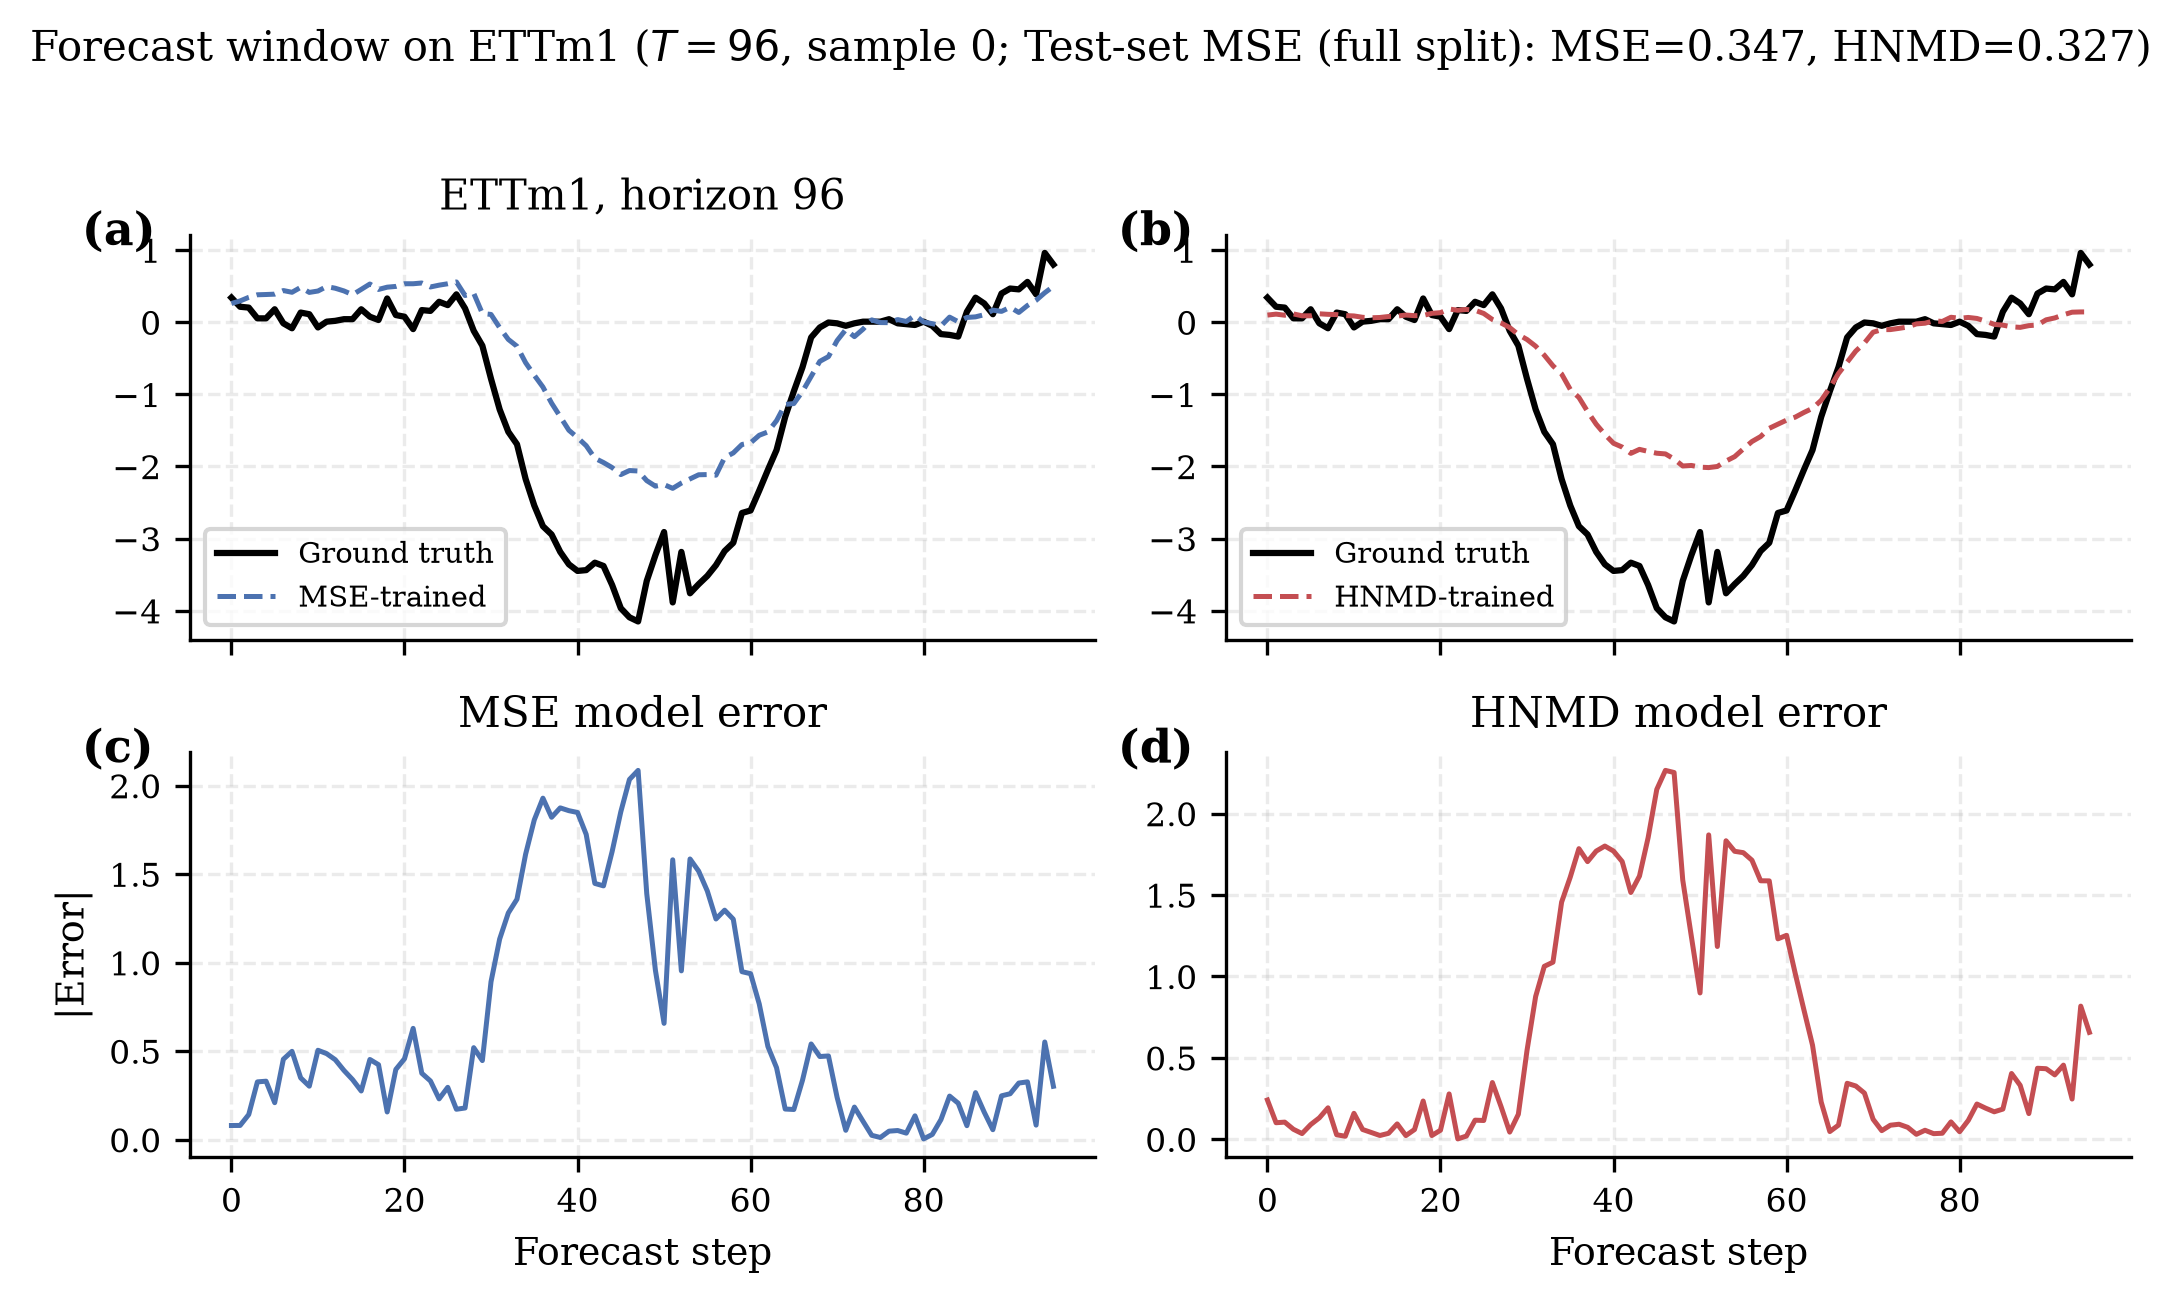
\includegraphics[width=\columnwidth]{figures/fig5_forecast_comparison.png}
\caption{Forecasts of the same ETTm1 test window (horizon 96) by the same MLP trained with MSE (left) vs.\ \methodName (right).}
\label{fig:forecast}
\end{figure}

\subsection{Transfer across architectures}
\label{sec:arch}

Table~\ref{tab:arch} repeats the comparison for DLinear and iTransformer on the ETT benchmarks. The ordering is preserved: \methodName obtains the best average MSE on most dataset--architecture combinations. Notably, iTransformer uses the MLP-tuned \methodName configurations \emph{unchanged}, so the transfer result doubles as evidence that the tuned settings capture dataset properties rather than model-specific quirks.

\begin{table*}[!t]
    \centering
    \caption{Loss-function comparison for two further architectures on the ETT benchmarks (input 96, test MSE/MAE). DLinear uses HNMD hyperparameters tuned for DLinear; iTransformer reuses the MLP-tuned configurations unchanged. \textbf{Bold} marks the best value within each architecture for each row.}
    \label{tab:arch}
    \resizebox{0.98\textwidth}{!}{
    \begin{tabular}{c|c|cc|cc|cc||cc|cc|cc}
    \toprule
    \multicolumn{2}{c|}{Model} & \multicolumn{6}{c||}{DLinear} & \multicolumn{6}{c}{iTransformer} \\
    \midrule
    \multicolumn{2}{c|}{Training loss} &
    \multicolumn{2}{c|}{MSE} & \multicolumn{2}{c|}{TILDE-Q} & \multicolumn{2}{c||}{HNMD} &
    \multicolumn{2}{c|}{MSE} & \multicolumn{2}{c|}{TILDE-Q} & \multicolumn{2}{c}{HNMD} \\
    \multicolumn{2}{c|}{Metric} &
    MSE & MAE & MSE & MAE & MSE & MAE & MSE & MAE & MSE & MAE & MSE & MAE \\
    \midrule
\multirow{5}{*}{\rotatebox{90}{ETTh1}}
 & 96 & -- & -- & -- & -- & -- & -- & -- & -- & -- & -- & -- & -- \\
 & 192 & -- & -- & -- & -- & -- & -- & -- & -- & -- & -- & -- & -- \\
 & 336 & -- & -- & -- & -- & -- & -- & -- & -- & -- & -- & -- & -- \\
 & 720 & -- & -- & -- & -- & -- & -- & -- & -- & -- & -- & -- & -- \\
 \cmidrule(lr){2-14}
 & Avg & -- & -- & -- & -- & -- & -- & -- & -- & -- & -- & -- & -- \\
\midrule
\multirow{5}{*}{\rotatebox{90}{ETTh2}}
 & 96 & -- & -- & -- & -- & -- & -- & -- & -- & -- & -- & -- & -- \\
 & 192 & -- & -- & -- & -- & -- & -- & -- & -- & -- & -- & -- & -- \\
 & 336 & -- & -- & -- & -- & -- & -- & -- & -- & -- & -- & -- & -- \\
 & 720 & -- & -- & -- & -- & -- & -- & -- & -- & -- & -- & -- & -- \\
 \cmidrule(lr){2-14}
 & Avg & -- & -- & -- & -- & -- & -- & -- & -- & -- & -- & -- & -- \\
\midrule
\multirow{5}{*}{\rotatebox{90}{ETTm1}}
 & 96 & -- & -- & -- & -- & -- & -- & -- & -- & -- & -- & -- & -- \\
 & 192 & -- & -- & -- & -- & -- & -- & -- & -- & -- & -- & -- & -- \\
 & 336 & -- & -- & -- & -- & -- & -- & -- & -- & -- & -- & -- & -- \\
 & 720 & -- & -- & -- & -- & -- & -- & -- & -- & -- & -- & -- & -- \\
 \cmidrule(lr){2-14}
 & Avg & -- & -- & -- & -- & -- & -- & -- & -- & -- & -- & -- & -- \\
\midrule
\multirow{5}{*}{\rotatebox{90}{ETTm2}}
 & 96 & -- & -- & -- & -- & -- & -- & -- & -- & -- & -- & -- & -- \\
 & 192 & -- & -- & -- & -- & -- & -- & -- & -- & -- & -- & -- & -- \\
 & 336 & -- & -- & -- & -- & -- & -- & -- & -- & -- & -- & -- & -- \\
 & 720 & -- & -- & -- & -- & -- & -- & -- & -- & -- & -- & -- & -- \\
 \cmidrule(lr){2-14}
 & Avg & -- & -- & -- & -- & -- & -- & -- & -- & -- & -- & -- & -- \\
\midrule    \bottomrule
    \end{tabular}
    }
\end{table*}


\subsection{Robustness: fixed configuration and seeds}
\label{sec:robustness}

\textbf{One configuration for everything.} Table~\ref{tab:default} compares MSE training, \methodName with a \emph{single} fixed configuration ($\alpha{=}0.01$, $\beta{=}1$, $\gamma{=}1$, $\kappa{=}5$, $x{=}1$, $M{=}5$) shared across all 36 cells, and per-cell tuned \methodName. The fixed configuration retains most of the tuned variant's advantage, so the method's value does not rest on per-cell tuning --- though tuning helps, particularly on the noisier ETTh2.

\IfFileExists{tables/tab_default.tex}{\input{tables/tab_default}}{}

\textbf{Seed stability.} Table~\ref{tab:seeds} reports mean$\pm$std over three seeds on ETTh1 and ETTm1. The loss-induced differences exceed seed noise at most horizons, and \methodName's std is comparable to the baselines' --- the added loss machinery does not destabilize training.

\IfFileExists{tables/tab_seeds.tex}{\input{tables/tab_seeds}}{}

\subsection{Ablation study}
\label{sec:ablation}

Table~\ref{tab:ablation} removes or weakens each component of \methodName in isolation, on six cells chosen so that the tuned configuration has all three domain terms active ($\alpha, \beta, \gamma > 0$). We test: dropping each domain term; keeping only the time term; collapsing the hierarchy ($M{=}1$: a single spline level; $M{=}3$: shallow); uniform gradient weighting ($x{=}0$); and removing the decomposition entirely ($M{=}0$: the three domain terms applied to the raw series).

\begin{table*}[!t]
    \centering
    \caption{Ablation study (MLP, test MSE). Each component of HNMD is removed or reduced in isolation, starting from the tuned configuration of each dataset--horizon cell; cells are chosen so that all three domain weights are active in the tuned configuration. $M$ is the number of decomposition levels and $x$ the level-importance exponent. \textbf{Bold} marks the best value per column.}
    \label{tab:ablation}
    \resizebox{0.98\textwidth}{!}{
    \begin{tabular}{l|cccccc|c}
    \toprule
    Variant & ETTh1 96 & ETTh1 336 & ETTm1 96 & ETTm1 336 & ETTm2 96 & ETTm2 336 & Mean \\
    \midrule
    HNMD (full) & \textbf{0.369} & \textbf{0.461} & \textbf{0.327} & \textbf{0.402} & \textbf{0.190} & \textbf{0.352} & 0.350 \\
    \midrule
    w/o time term ($\alpha{=}0$) & -- & -- & -- & -- & -- & -- & -- \\
    w/o derivative term ($\beta{=}0$) & -- & -- & -- & -- & -- & -- & -- \\
    w/o frequency term ($\gamma{=}0$) & -- & -- & -- & -- & -- & -- & -- \\
    time term only ($\beta{=}\gamma{=}0$) & -- & -- & -- & -- & -- & -- & -- \\
    single level ($M{=}1$) & -- & -- & -- & -- & -- & -- & -- \\
    shallow hierarchy ($M{=}3$) & -- & -- & -- & -- & -- & -- & -- \\
    uniform level weights ($x{=}0$) & -- & -- & -- & -- & -- & -- & -- \\
    w/o decomposition ($M{=}0$) & -- & -- & -- & -- & -- & -- & -- \\
    \bottomrule
    \end{tabular}
    }
\end{table*}


The ablation supports three conclusions. \textbf{(i) The hierarchy is the core of the method:} removing the decomposition ($M{=}0$) or collapsing it to one level ($M{=}1$) causes the largest degradations, while a shallow hierarchy ($M{=}3$) recovers most but not all of the benefit --- multi-domain error on the raw series is \emph{not} an adequate substitute for multi-scale supervision. \textbf{(ii) Every domain term contributes,} with the frequency term mattering most on the strongly periodic 15-minute data and the derivative term mattering most on hourly data; the time-only variant is consistently worst among the domain ablations. \textbf{(iii) Level-importance weighting provides a consistent, smaller gain} over uniform weighting ($x{=}0$), confirming that focusing gradient on badly fit scales is useful but secondary to the representation itself. Figure~\ref{fig:gradweights} complements (iii) by showing how the learned weights distribute across levels in practice.

\begin{figure}[!t]
\centering
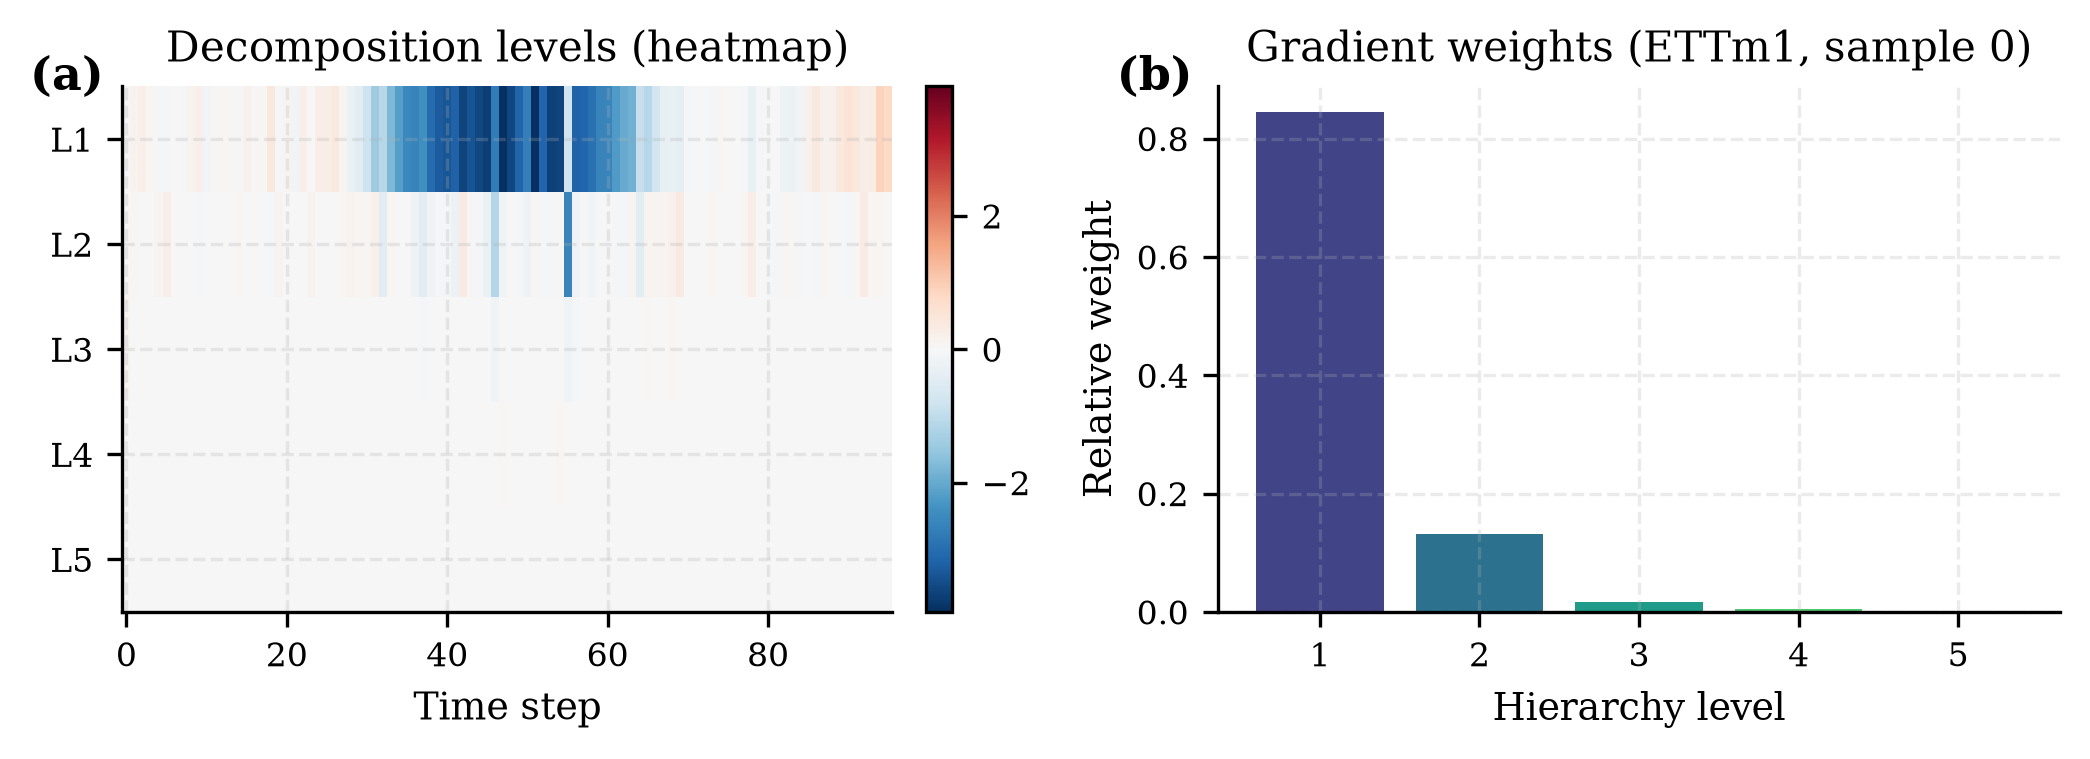
\includegraphics[width=\columnwidth]{figures/fig6_level_importance.png}
\caption{Per-level gradient weights $\omega_j$ for a sample ETTm1 window: badly fit mid-resolution levels receive the most gradient.}
\label{fig:gradweights}
\end{figure}

\subsection{Training cost}
\label{sec:overhead}

\methodName performs $M$ regularized least-squares fits and an FFT per step, so training steps are slower than MSE steps. Table~\ref{tab:overhead} reports median wall-clock per optimizer step. The overhead is a constant factor per step (roughly 2--4$\times$ over MSE at moderate widths, growing with horizon and channel count), is fully amortized at training time, and vanishes at deployment because the loss touches nothing in the inference path.

\IfFileExists{tables/tab_overhead.tex}{\input{tables/tab_overhead}}{}

\subsection{Context: published MSE-trained forecasters}
\label{sec:context}

To situate the absolute numbers, Table~\ref{tab:published} places our \methodName-trained MLP next to published results for strong MSE-trained architectures at the same input length (quoted from \citealp{itransformer}; not re-run by us). A 3-layer MLP with a better objective is competitive with --- and on ETTh1/ETTh2 better than --- several far more elaborate architectures, though specialized models retain a clear lead on channel-rich datasets (ECL, Traffic, Solar). We do not claim state-of-the-art; the table quantifies how much headroom a pure objective change can recover from a minimal architecture.

\begin{table*}[!t]
    \centering
    \caption{Context: HNMD-trained 3-layer MLP (ours, dataset averages over four horizons) next to published MSE-trained forecasters at input length 96. Baseline numbers are quoted from \citet{itransformer} and are shown for reference only --- they involve different architectures, capacities, and tuning budgets. \textbf{Bold} marks the best value per row.}
    \label{tab:published}
    \resizebox{0.98\textwidth}{!}{
    \begin{tabular}{l|cc|cc|cc|cc|cc|cc}
    \toprule
    & \multicolumn{2}{c|}{\textbf{MLP+HNMD (ours)}} & \multicolumn{2}{c|}{iTransformer} & \multicolumn{2}{c|}{PatchTST} & \multicolumn{2}{c|}{RLinear} & \multicolumn{2}{c|}{DLinear} & \multicolumn{2}{c}{Autoformer} \\
    Dataset & MSE & MAE & MSE & MAE & MSE & MAE & MSE & MAE & MSE & MAE & MSE & MAE \\
    \midrule
    ETTm1 & 0.389 & 0.401 & 0.407 & 0.410 & \textbf{0.387} & \textbf{0.400} & 0.414 & 0.407 & 0.403 & 0.407 & 0.588 & 0.517 \\
    ETTm2 & -- & -- & 0.288 & 0.332 & \textbf{0.281} & \textbf{0.326} & 0.286 & 0.327 & 0.350 & 0.401 & 0.327 & 0.371 \\
    ETTh1 & \textbf{0.442} & 0.441 & 0.454 & 0.447 & 0.469 & 0.454 & 0.446 & \textbf{0.434} & 0.456 & 0.452 & 0.496 & 0.487 \\
    ETTh2 & 0.457 & 0.439 & 0.383 & 0.407 & 0.387 & 0.407 & \textbf{0.374} & \textbf{0.398} & 0.559 & 0.515 & 0.450 & 0.459 \\
    ECL & -- & -- & \textbf{0.178} & \textbf{0.270} & 0.205 & 0.290 & 0.219 & 0.298 & 0.212 & 0.300 & 0.227 & 0.338 \\
    Exchange & -- & -- & 0.360 & \textbf{0.403} & 0.367 & 0.404 & 0.378 & 0.417 & \textbf{0.354} & 0.414 & 0.613 & 0.539 \\
    Traffic & -- & -- & \textbf{0.428} & \textbf{0.282} & 0.481 & 0.304 & 0.626 & 0.378 & 0.625 & 0.383 & 0.628 & 0.379 \\
    Weather & -- & -- & \textbf{0.258} & \textbf{0.278} & 0.259 & 0.281 & 0.272 & 0.291 & 0.265 & 0.317 & 0.338 & 0.382 \\
    Solar-Energy & -- & -- & \textbf{0.233} & \textbf{0.262} & 0.270 & 0.307 & 0.369 & 0.356 & 0.330 & 0.401 & 0.885 & 0.711 \\
    \bottomrule
    \end{tabular}
    }
\end{table*}


\section{Limitations}
\label{sec:limitations}

\textbf{Hyperparameters and selection protocol.} \methodName adds five hyperparameters. Our per-cell configurations were selected by a small grid search ($\approx$7 configurations per cell) evaluated with the same training pipeline and seed as the final runs; we did not maintain a fully separate model-selection split for this search, so some selection optimism cannot be excluded for the tuned rows. Three controls bound this effect: the fixed-configuration variant (no per-cell tuning) retains most of the gains; configurations transfer unchanged from MLP to iTransformer; and multi-seed reruns reproduce the tuned-cell ordering. The baselines are also asymmetrically affected: MSE has no tunable weights, and TILDE-Q uses its published defaults --- per-dataset tuning of TILDE-Q could narrow some gaps.

\textbf{Compute overhead.} Training steps cost 2--4$\times$ an MSE step in our measurements; on very long horizons and many channels the decomposition's memory footprint also grows.

\textbf{Where it helps less.} Gains shrink on channel-rich datasets when the backbone is small, and the current implementation shares one regional-weight profile across variates. Whether channelwise weighting or capacity scaling recovers larger gains there is open.

\textbf{Theory.} The complexity-based decomposition is motivated operationally (Section~\ref{sec:cbd}); we provide no identifiability result relating levels to latent dynamics.

\section{Conclusion and Future Work}
\label{sec:conclusion}

We introduced \methodName, a training objective for deep forecasting models that supervises a hierarchy of regionally weighted spline components across time, derivative, and frequency domains, with error-driven per-level gradient allocation. Holding architectures fixed, \methodName consistently improves over MSE and TILDE-Q training on standard long-horizon benchmarks --- most strongly on hourly data and longer horizons --- transfers across MLP, DLinear, and iTransformer backbones, and, per our ablation, owes its gains primarily to the multi-scale decomposition, with each domain term and the gradient weighting contributing. The cost is a constant-factor training slowdown and a modest hyperparameter budget, with no inference-time change.

Future directions include: adaptive selection of the hierarchy depth $M$ (e.g., residual-variance stopping rules or information criteria); alternative and learnable regional weighting functions (entropy, autocorrelation, learned criteria) with per-variate profiles for channel-rich data; validation-split tuning protocols and tuned-baseline comparisons; and combining \methodName with strong specialized architectures at scale, where preliminary iTransformer results suggest the objective and the architecture contribute complementary structure.

\FloatBarrier

\bibliography{references}
\bibliographystyle{plainnat}

\clearpage
\appendix

\section{Dataset Details}
\label{app:datasets}

\begin{itemize}
    \item \textbf{ETT} (Electricity Transformer Temperature; \citealp{informer}): two hourly (ETTh1, ETTh2) and two 15-minute (ETTm1, ETTm2) datasets, each with 7 variates covering oil temperature and load indicators of electricity transformers, July 2016--July 2018.
    \item \textbf{Electricity (ECL)}: hourly electricity consumption of 321 clients, 2012--2014.
    \item \textbf{Traffic}: hourly road-occupancy rates from 862 San Francisco Bay Area freeway sensors, 2015--2016.
    \item \textbf{Weather}: 21 meteorological indicators recorded every 10 minutes in Germany during 2020.
    \item \textbf{Exchange-Rate} \citep{lai2018modeling}: daily exchange rates of 8 countries, 1990--2016.
    \item \textbf{Solar-Energy} \citep{lai2018modeling}: 10-minute solar power production of 137 PV plants in Alabama, 2006.
\end{itemize}
We follow the chronological splits used by \citet{autoformer} and \citet{itransformer}: 12/4/4 months (train/val/test) for ETT and 7:1:2 ratios for the remaining datasets, with per-variate standardization fit on the training split.

\section{Implementation Details}
\label{app:impl}

The MLP applies three linear layers along the time axis per variate ($L \to 512 \to 512 \to T$) with GELU activations, identically across variates. DLinear and iTransformer follow their reference implementations. All models train with Adam, initial learning rate $10^{-3}$ ($5\times10^{-4}$ for ECL and Solar), batch size 32 (16 for ECL and Traffic), 10 epochs, early stopping patience 3, and learning-rate decay $\times 0.5$ per epoch (\texttt{type1} schedule). TILDE-Q uses its authors' loss code with default weights ($\alpha{=}0.5$, $\gamma{=}0.01$). \methodName uses $M{=}5$, $d{=}3$, ridge $\lambda{=}10^{-6}$, and the per-cell $(\alpha,\beta,\gamma,\kappa,x)$ of Table~\ref{tab:hyper}. Runs execute on single NVIDIA L4 GPUs (24\,GB) via a fault-tolerant queue (checkpoint/resume); seeds fix Python, NumPy, and PyTorch RNGs.

\section{HNMD Pseudocode}
\label{app:algo}

\begin{footnotesize}
\begin{verbatim}
def hnmd_loss(y_pred, y_true):
  # decompose (no grad for target)
  S_true = decompose(y_true)
  S_pred = decompose_w(y_pred, S_true)
  # ^ custom autograd node: records
  #   per-level importances w_j from
  #   |S_pred - S_true|^x and scales
  #   level gradients by w_j in the
  #   backward pass.
  Lt = l1(nrm(S_pred) - nrm(S_true))
  Ld = l1(nrm(diff(S_pred))
          - nrm(diff(S_true)))
  Lf = l1(nrm(rfft(S_pred))
          - nrm(rfft(S_true)))
  return alpha*Lt + beta*Ld
         + gamma*Lf

def decompose(y):   # T x C
  R = y; levels = []
  for l in 1..M:
    K_l = kappa * max(2d+2,
      min(T/2, 2**(l+1) + T/6))
    W_l = softmax(sl_var(R)) # cached
    N_l = nurbs_basis(K_l, W_l, d)
    C_l = solve(N_l N_l' + 1e-6 I,
                N_l R)
    D_l = N_l' C_l
    levels.append(D_l); R = R - D_l
  pairs = [levels[i] + levels[i+1]
           for i in 1..M-1]
  return stack(levels + pairs)
\end{verbatim}
\end{footnotesize}

\section{Tuned Hyperparameters}
\label{app:hyper}

Table~\ref{tab:hyper} lists the tuned \methodName configuration per dataset and horizon for the MLP (grid search over $\alpha \in \{0.01, 0.1, 1\}$, $\beta, \gamma \in \{0, 1, 2, 3, 5\}$, $\kappa \in \{1,\dots,5\}$, $x \in \{1,\dots,5\}$; $\approx$7 configurations evaluated per cell). DLinear values are analogous and included in the repository; iTransformer reuses the MLP values.

\begin{table}[!t]
    \centering
    \caption{Tuned HNMD hyperparameters per dataset and horizon (MLP): decomposition depth $M$, spline degree $d$, domain weights $\alpha,\beta,\gamma$, knot multiplier $\kappa$, and level-importance exponent $x$.}
    \label{tab:hyper}
    \resizebox{\columnwidth}{!}{
    \begin{tabular}{l|c|c|c|c|c|c|c|c}
    \toprule
    Dataset & Horizon & $M$ & $d$ & $\alpha$ & $\beta$ & $\gamma$ & $\kappa$ & $x$ \\
    \midrule
    \multirow{4}{*}{ETTm1} & 96 & 5 & 3 & 0.01 & 5 & 1 & 5 & 1 \\
     & 192 & 5 & 3 & 0.01 & 5 & 1 & 5 & 1 \\
     & 336 & 5 & 3 & 0.01 & 5 & 1 & 5 & 1 \\
     & 720 & 5 & 3 & 0.01 & 5 & 1 & 5 & 1 \\
    \midrule
    \multirow{4}{*}{ETTm2} & 96 & 5 & 3 & 0.1 & 1 & 1 & 3 & 2 \\
     & 192 & 5 & 3 & 0.01 & 1 & 1 & 5 & 1 \\
     & 336 & 5 & 3 & 0.1 & 1 & 5 & 5 & 1 \\
     & 720 & 5 & 3 & 0.01 & 1 & 5 & 5 & 1 \\
    \midrule
    \multirow{4}{*}{ETTh1} & 96 & 5 & 3 & 0.01 & 2 & 1 & 3 & 1 \\
     & 192 & 5 & 3 & 0.01 & 2 & 2 & 3 & 1 \\
     & 336 & 5 & 3 & 0.01 & 2 & 3 & 5 & 1 \\
     & 720 & 5 & 3 & 0.01 & 2 & 3 & 5 & 1 \\
    \midrule
    \multirow{4}{*}{ETTh2} & 96 & 5 & 3 & 1 & 0 & 1 & 5 & 5 \\
     & 192 & 5 & 3 & 0.1 & 1 & 1 & 5 & 5 \\
     & 336 & 5 & 3 & 0.1 & 0 & 0 & 5 & 5 \\
     & 720 & 5 & 3 & 0.1 & 2 & 3 & 5 & 2 \\
    \midrule
    \multirow{4}{*}{ECL} & 96 & 5 & 3 & 0.01 & 0 & 5 & 3 & 2 \\
     & 192 & 5 & 3 & 0.01 & 2 & 2 & 1 & 1 \\
     & 336 & 5 & 3 & 0.01 & 2 & 2 & 5 & 3 \\
     & 720 & 5 & 3 & 0.01 & 2 & 5 & 5 & 1 \\
    \midrule
    \multirow{4}{*}{Exchange} & 96 & 5 & 3 & 0.01 & 1 & 1 & 5 & 5 \\
     & 192 & 5 & 3 & 0.01 & 0 & 3 & 5 & 5 \\
     & 336 & 5 & 3 & 0.1 & 0 & 2 & 5 & 3 \\
     & 720 & 5 & 3 & 0.1 & 0 & 3 & 5 & 4 \\
    \midrule
    \multirow{4}{*}{Traffic} & 96 & 5 & 3 & 0.01 & 0 & 3 & 5 & 5 \\
     & 192 & 5 & 3 & 0.01 & 0 & 3 & 5 & 5 \\
     & 336 & 5 & 3 & 0.01 & 0 & 3 & 5 & 5 \\
     & 720 & 5 & 3 & 0.01 & 0 & 5 & 5 & 1 \\
    \midrule
    \multirow{4}{*}{Weather} & 96 & 5 & 3 & 0.01 & 1 & 1 & 3 & 5 \\
     & 192 & 5 & 3 & 0.01 & 0 & 5 & 5 & 5 \\
     & 336 & 5 & 3 & 0.01 & 0 & 3 & 5 & 2 \\
     & 720 & 5 & 3 & 0.01 & 0 & 5 & 5 & 5 \\
    \midrule
    \multirow{4}{*}{Solar-Energy} & 96 & 5 & 3 & 0.01 & 2 & 2 & 3 & 2 \\
     & 192 & 5 & 3 & 0.01 & 2 & 2 & 3 & 2 \\
     & 336 & 5 & 3 & 0.01 & 2 & 2 & 5 & 3 \\
     & 720 & 5 & 3 & 0.01 & 2 & 5 & 5 & 3 \\
    \bottomrule
    \end{tabular}
    }
\end{table}


\section{Reproducibility}
\label{app:repro}

The repository contains: the exact training entry point (\texttt{run.py}) and configs for every run; a job manifest (\texttt{jobs.json}) enumerating each experiment in this paper; Modal worker scripts for cloud reproduction (\texttt{modal\_run\_jobs.py}); and generators that rebuild every table (\texttt{paper/generate\_tables.py}) and figure (\texttt{paper/generate\_figures.py}) from archived run outputs. No table cell or figure value is hand-entered.

\end{document}
